% -----------------------------------------------------------------------
% CHAPITRE 3 - RESULTATS : clustering K=6 + regles d'association (Boeny)
% -----------------------------------------------------------------------
% A inclure dans votre .tex principal avec % -----------------------------------------------------------------------
% CHAPITRE 3 - RESULTATS : clustering K=6 + regles d'association (Boeny)
% -----------------------------------------------------------------------
% A inclure dans votre .tex principal avec % -----------------------------------------------------------------------
% CHAPITRE 3 - RESULTATS : clustering K=6 + regles d'association (Boeny)
% -----------------------------------------------------------------------
% A inclure dans votre .tex principal avec % -----------------------------------------------------------------------
% CHAPITRE 3 - RESULTATS : clustering K=6 + regles d'association (Boeny)
% -----------------------------------------------------------------------
% A inclure dans votre .tex principal avec \input{chapitre3_resultats_clustering.tex}.
% Donnees : trajectoires_avec_clusters.csv (482 359 cellules), K=6, silhouette 0,765.
% Compilation : pdflatex (ou lualatex) + biblatex. Figures fournies par
% visualisation_spatiale_boeny.py / clustering_regles_association_boeny.py.
% -----------------------------------------------------------------------

\chapter{Résultats : dynamique spatio-temporelle du Boeny (2016--2025)}
\label{ch:resultats}

\section{Partition en six trajectoires types}

L'agrégation des rasters Dynamics World à 10 m vers une résolution de 250 m a
produit \numprint{482359} cellules valides sur la période 2016--2025 (masque
polygone appliqué, EPSG:32738). Après lissage (fenêtre $3\times3$ + médian
temporel, bruit ramené de \SI{16,4}{\percent} à \SI{2,0}{\percent}), un
k-means à $K=6$ — justifié par la convergence du coude d'inertie
($-20{,}7\,\%$ de 5 à 6) et de la silhouette de Rousseeuw maximale
($s=\numprint{0,765}$) — a été appliqué. La répartition est la suivante :

\begin{table}[H]
\centering
\caption{Répartition des cellules par cluster (k-means, $K=6$, 
$n_{\text{start}}=25$, silhouette $0{,}765$).}
\label{tab:repartition_clusters}
\begin{tabular}{lrrrl}
\toprule
Cluster & Cellules & \multicolumn{1}{c}{\%} & Silhouette & Lecture \\
\midrule
1 & \numprint{12909} & 2{,}7 & 0{,}166 & Eau stable (vasières / estuaire) \\
2 & \numprint{17996} & 3{,}7 & 0{,}418 & Cultures / sol nu (agriculture) \\
3 & \numprint{73390} & 15{,}2 & 0{,}796 & Transition forêt--savane (dynamique) \\
4 & \numprint{8228} & 1{,}7 & 0{,}258 & Végétation inondée (côte) \\
5 & \numprint{269063} & 55{,}8 & 0{,}000 & Savane stable \\
6 & \numprint{100773} & 20{,}9 & 0{,}000 & Forêt stable \\
\midrule
Total & \numprint{482359} & 100 & --- & --- \\
\bottomrule
\end{tabular}
\end{table}

\begin{figure}[H]
\centering
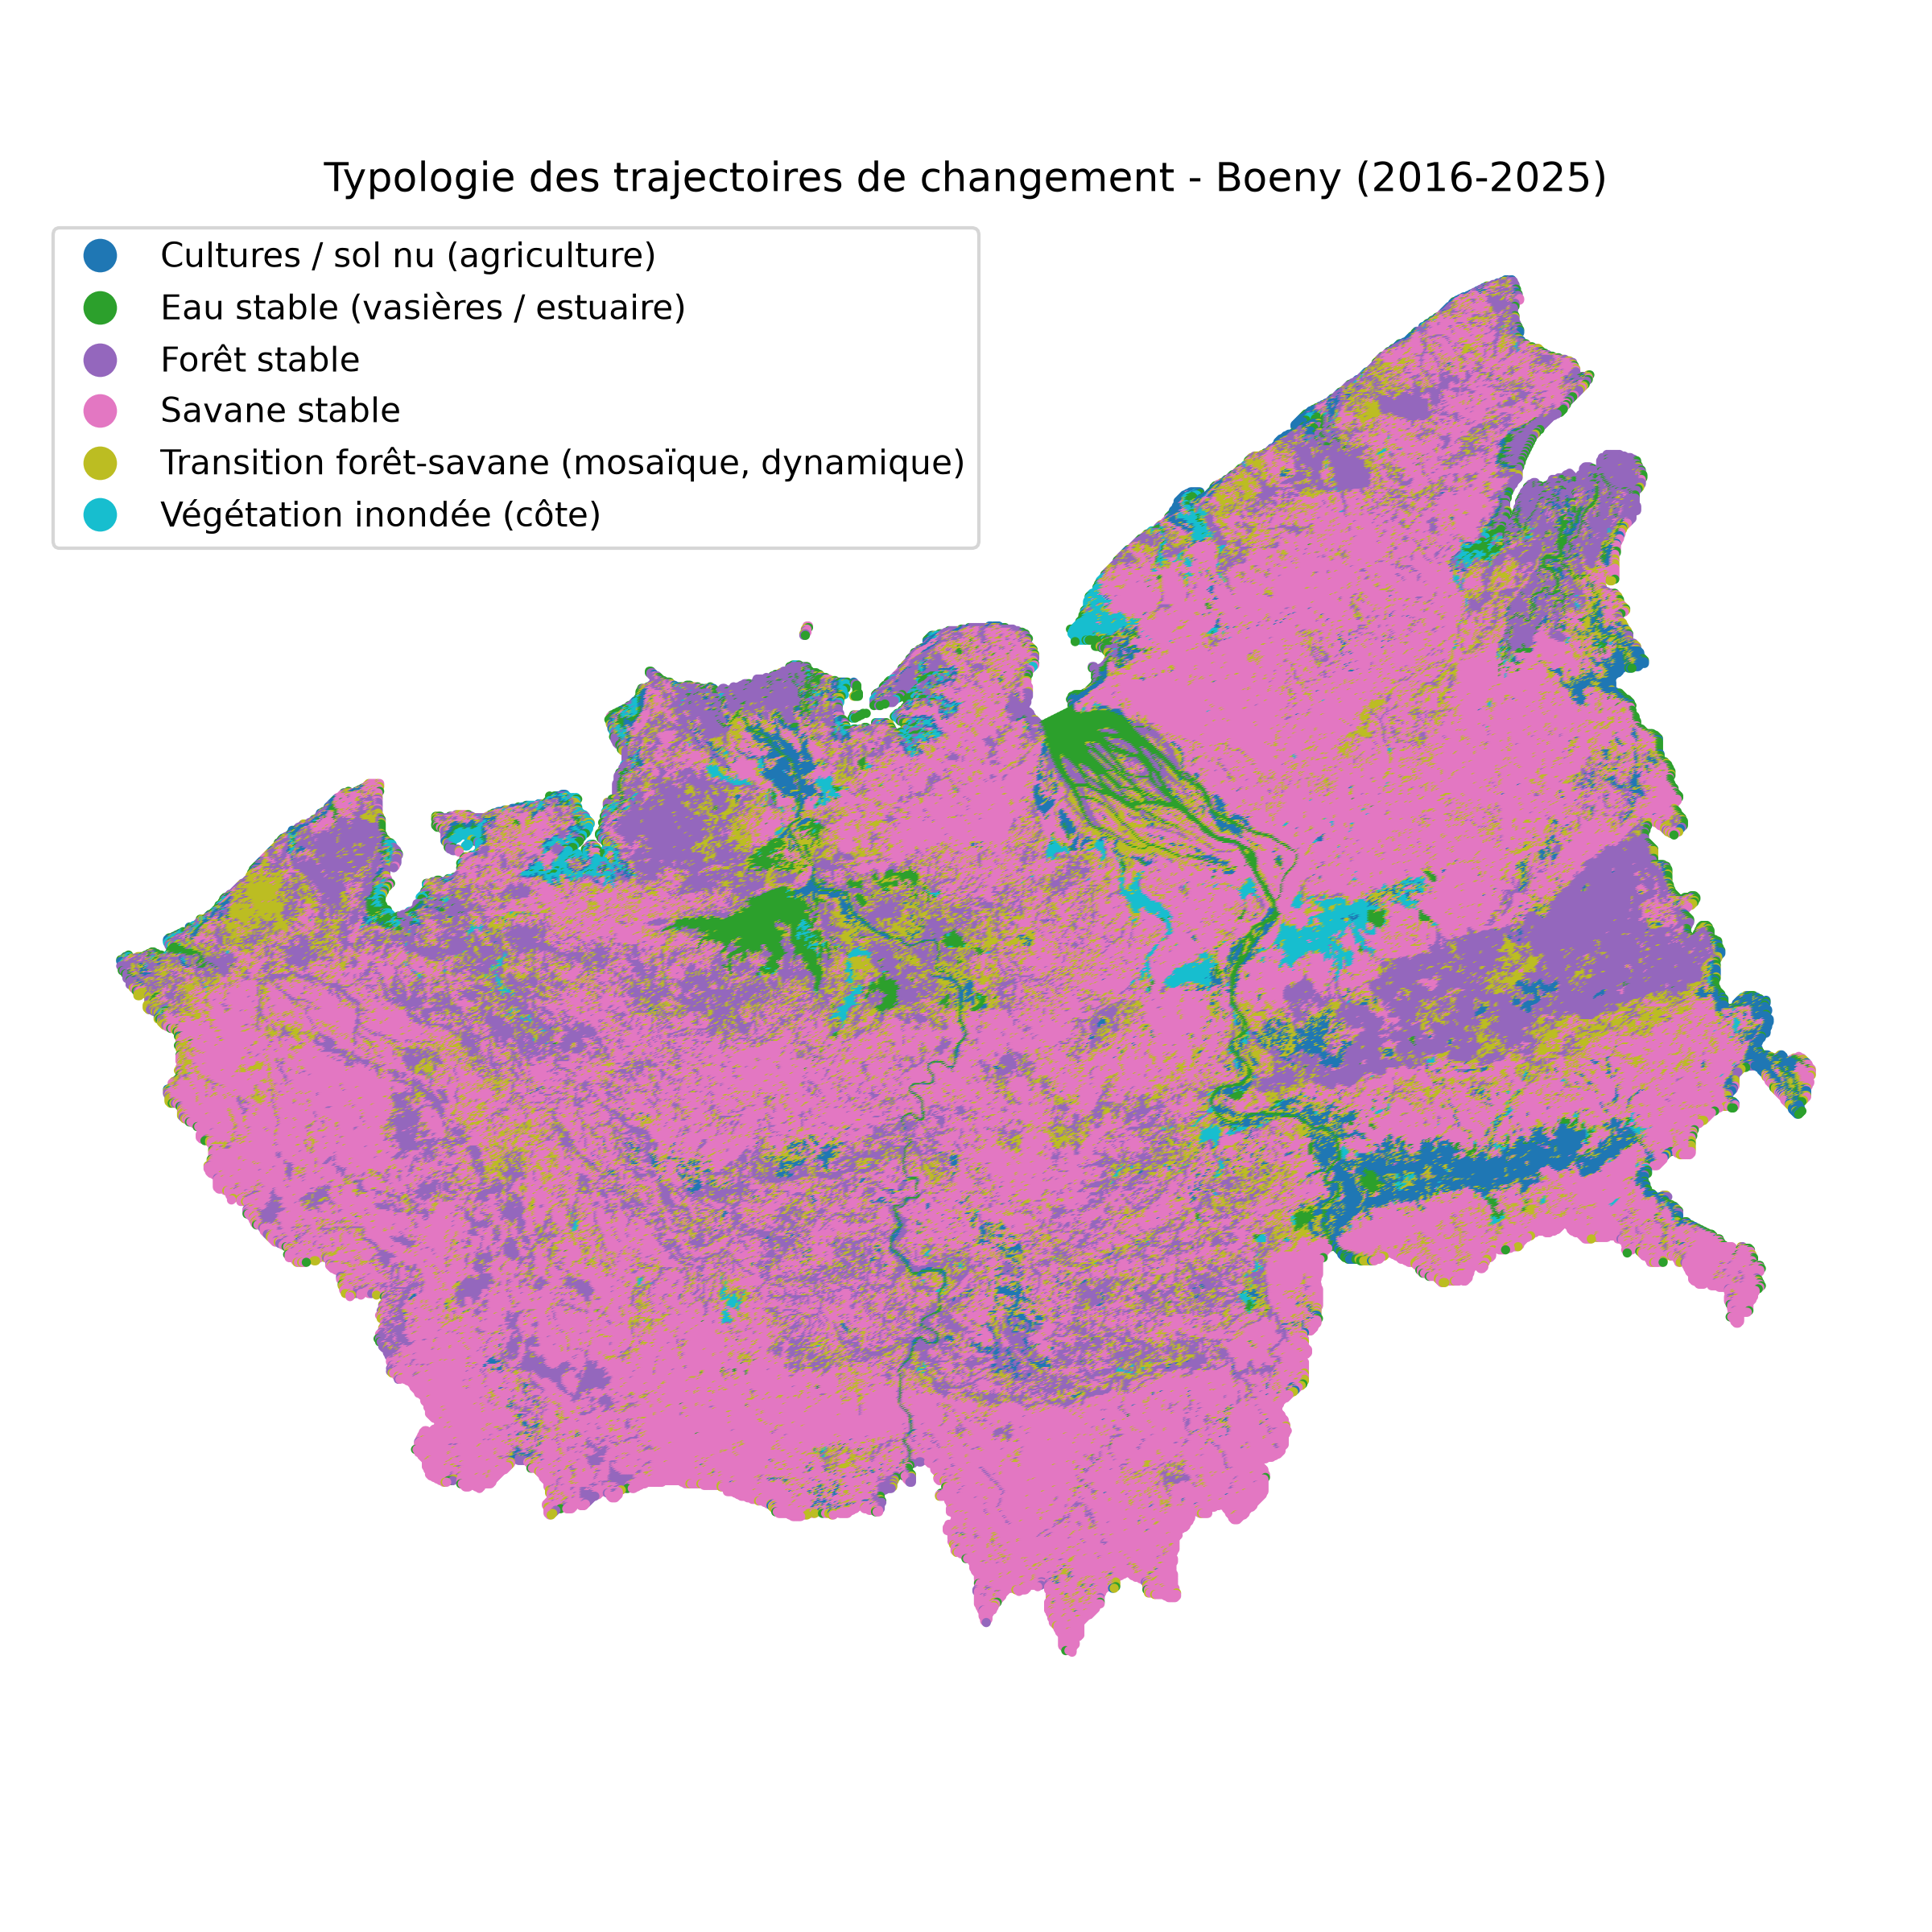
\includegraphics[width=0.85\textwidth]{carte_clusters_trajectoires.png}
\caption{Carte des trajectoires de changement (Boeny, 2016--2025), 6 clusters.}
\label{fig:carte_clusters}
\end{figure}

\section{Règles d'association sur les transitions}

L'extraction Apriori (support $\geq 0{,}01$, confiance $\geq 0{,}5$, tri par
lift) a produit 10 règles sur les \numprint{86988} cellules présentant au
moins une transition. Les plus informatives traduisent des dynamiques
spatialement localisées :

\begin{table}[H]
\centering
\caption{Principales règles d'association (extrait, tri par lift).}
\label{tab:regles_association}
\begin{tabular}{lrrrll}
\toprule
Règle (lhs $\Rightarrow$ rhs) & Support & Confiance & Lift & Effectif & Lecture \\
\midrule
eau $\Leftrightarrow$ sol nu & 0{,}010 & 0{,}56--0{,}65 & \numprint{34,9} & 899 & Vasières / estuaire (alternance annuelle) \\
vég. inondée $\Leftrightarrow$ vég. non for. & 0{,}011 & 0{,}53 & \numprint{26,7} & 914 & Frange littorale humide \\
vég. inondée $\Leftrightarrow$ forêt & 0{,}012 & 0{,}53 & \numprint{22,3} & 1007 & Bordure forêt / zone inondée \\
cultures $\Leftrightarrow$ vég. non for. & 0{,}062 & 0{,}54--0{,}62 & \numprint{5,4} & 5380 & \textbf{Front agricole} \\
forêt $\Leftrightarrow$ vég. non for. & 0{,}268 & 0{,}54--0{,}60 & \numprint{1,2} & 23307 & Co-occurrence (lift $\approx 1$, peu informative) \\
\bottomrule
\end{tabular}
\end{table}

% --- Resultat clé à mettre en avant --------------------------------
\subsection{À retenir pour le mémoire}

Deux résultats structurent le chapitre~3 : (i) l'association
\textbf{eau $\Leftrightarrow$ sol nu} (lift \numprint{34,9}) caractérise les
vasières de l'estuaire de la Betsiboka, où le marnage fait osciller la classe
d'occupation d'une année à l'autre — une dynamique côtière \emph{localisée et
intense} ; (ii) l'association \textbf{cultures $\Leftrightarrow$ vég. non
forestière} (lift \numprint{5,4}, support \SI{6,2}{\percent}) matérialise le
front agricole en bordure des espaces naturels. La règle
\textbf{forêt $\Leftrightarrow$ vég. non forestière}, bien que la plus
volumineuse (support \SI{26,8}{\percent}), est la moins informative
(lift $\approx 1{,}2$ $\approx$ indépendance) : son interprétation en terme de
dynamique doit être évitée — c'est une \emph{co-occurrence spatiale} de la
mosaïque forêt--savane à l'échelle 250 m.

% --- Section méthodologique (reproductibilité) ----------------------
\section{Reproductibilité}

L'ensemble du pipeline est reproducible avec une graine fixe
($\texttt{SEED}=1$, $\texttt{random\_state}=1$, $\texttt{nstart}=25$) et les
commandes documentées dans \texttt{GUIDE\_EXECUTION.md}. La silhouette est
calculée sur un échantillon de \numprint{5000} cellules (pratique standard en
raison du coût $O(n^2)$ du calcul complet). Le choix de $K=6$ maximise
simultanément la silhouette (\numprint{0,765}) et se situe au dernier coude
d'inertie stabilisé — deux critères indépendants convergent.

.
% Donnees : trajectoires_avec_clusters.csv (482 359 cellules), K=6, silhouette 0,765.
% Compilation : pdflatex (ou lualatex) + biblatex. Figures fournies par
% visualisation_spatiale_boeny.py / clustering_regles_association_boeny.py.
% -----------------------------------------------------------------------

\chapter{Résultats : dynamique spatio-temporelle du Boeny (2016--2025)}
\label{ch:resultats}

\section{Partition en six trajectoires types}

L'agrégation des rasters Dynamics World à 10 m vers une résolution de 250 m a
produit \numprint{482359} cellules valides sur la période 2016--2025 (masque
polygone appliqué, EPSG:32738). Après lissage (fenêtre $3\times3$ + médian
temporel, bruit ramené de \SI{16,4}{\percent} à \SI{2,0}{\percent}), un
k-means à $K=6$ — justifié par la convergence du coude d'inertie
($-20{,}7\,\%$ de 5 à 6) et de la silhouette de Rousseeuw maximale
($s=\numprint{0,765}$) — a été appliqué. La répartition est la suivante :

\begin{table}[H]
\centering
\caption{Répartition des cellules par cluster (k-means, $K=6$, 
$n_{\text{start}}=25$, silhouette $0{,}765$).}
\label{tab:repartition_clusters}
\begin{tabular}{lrrrl}
\toprule
Cluster & Cellules & \multicolumn{1}{c}{\%} & Silhouette & Lecture \\
\midrule
1 & \numprint{12909} & 2{,}7 & 0{,}166 & Eau stable (vasières / estuaire) \\
2 & \numprint{17996} & 3{,}7 & 0{,}418 & Cultures / sol nu (agriculture) \\
3 & \numprint{73390} & 15{,}2 & 0{,}796 & Transition forêt--savane (dynamique) \\
4 & \numprint{8228} & 1{,}7 & 0{,}258 & Végétation inondée (côte) \\
5 & \numprint{269063} & 55{,}8 & 0{,}000 & Savane stable \\
6 & \numprint{100773} & 20{,}9 & 0{,}000 & Forêt stable \\
\midrule
Total & \numprint{482359} & 100 & --- & --- \\
\bottomrule
\end{tabular}
\end{table}

\begin{figure}[H]
\centering
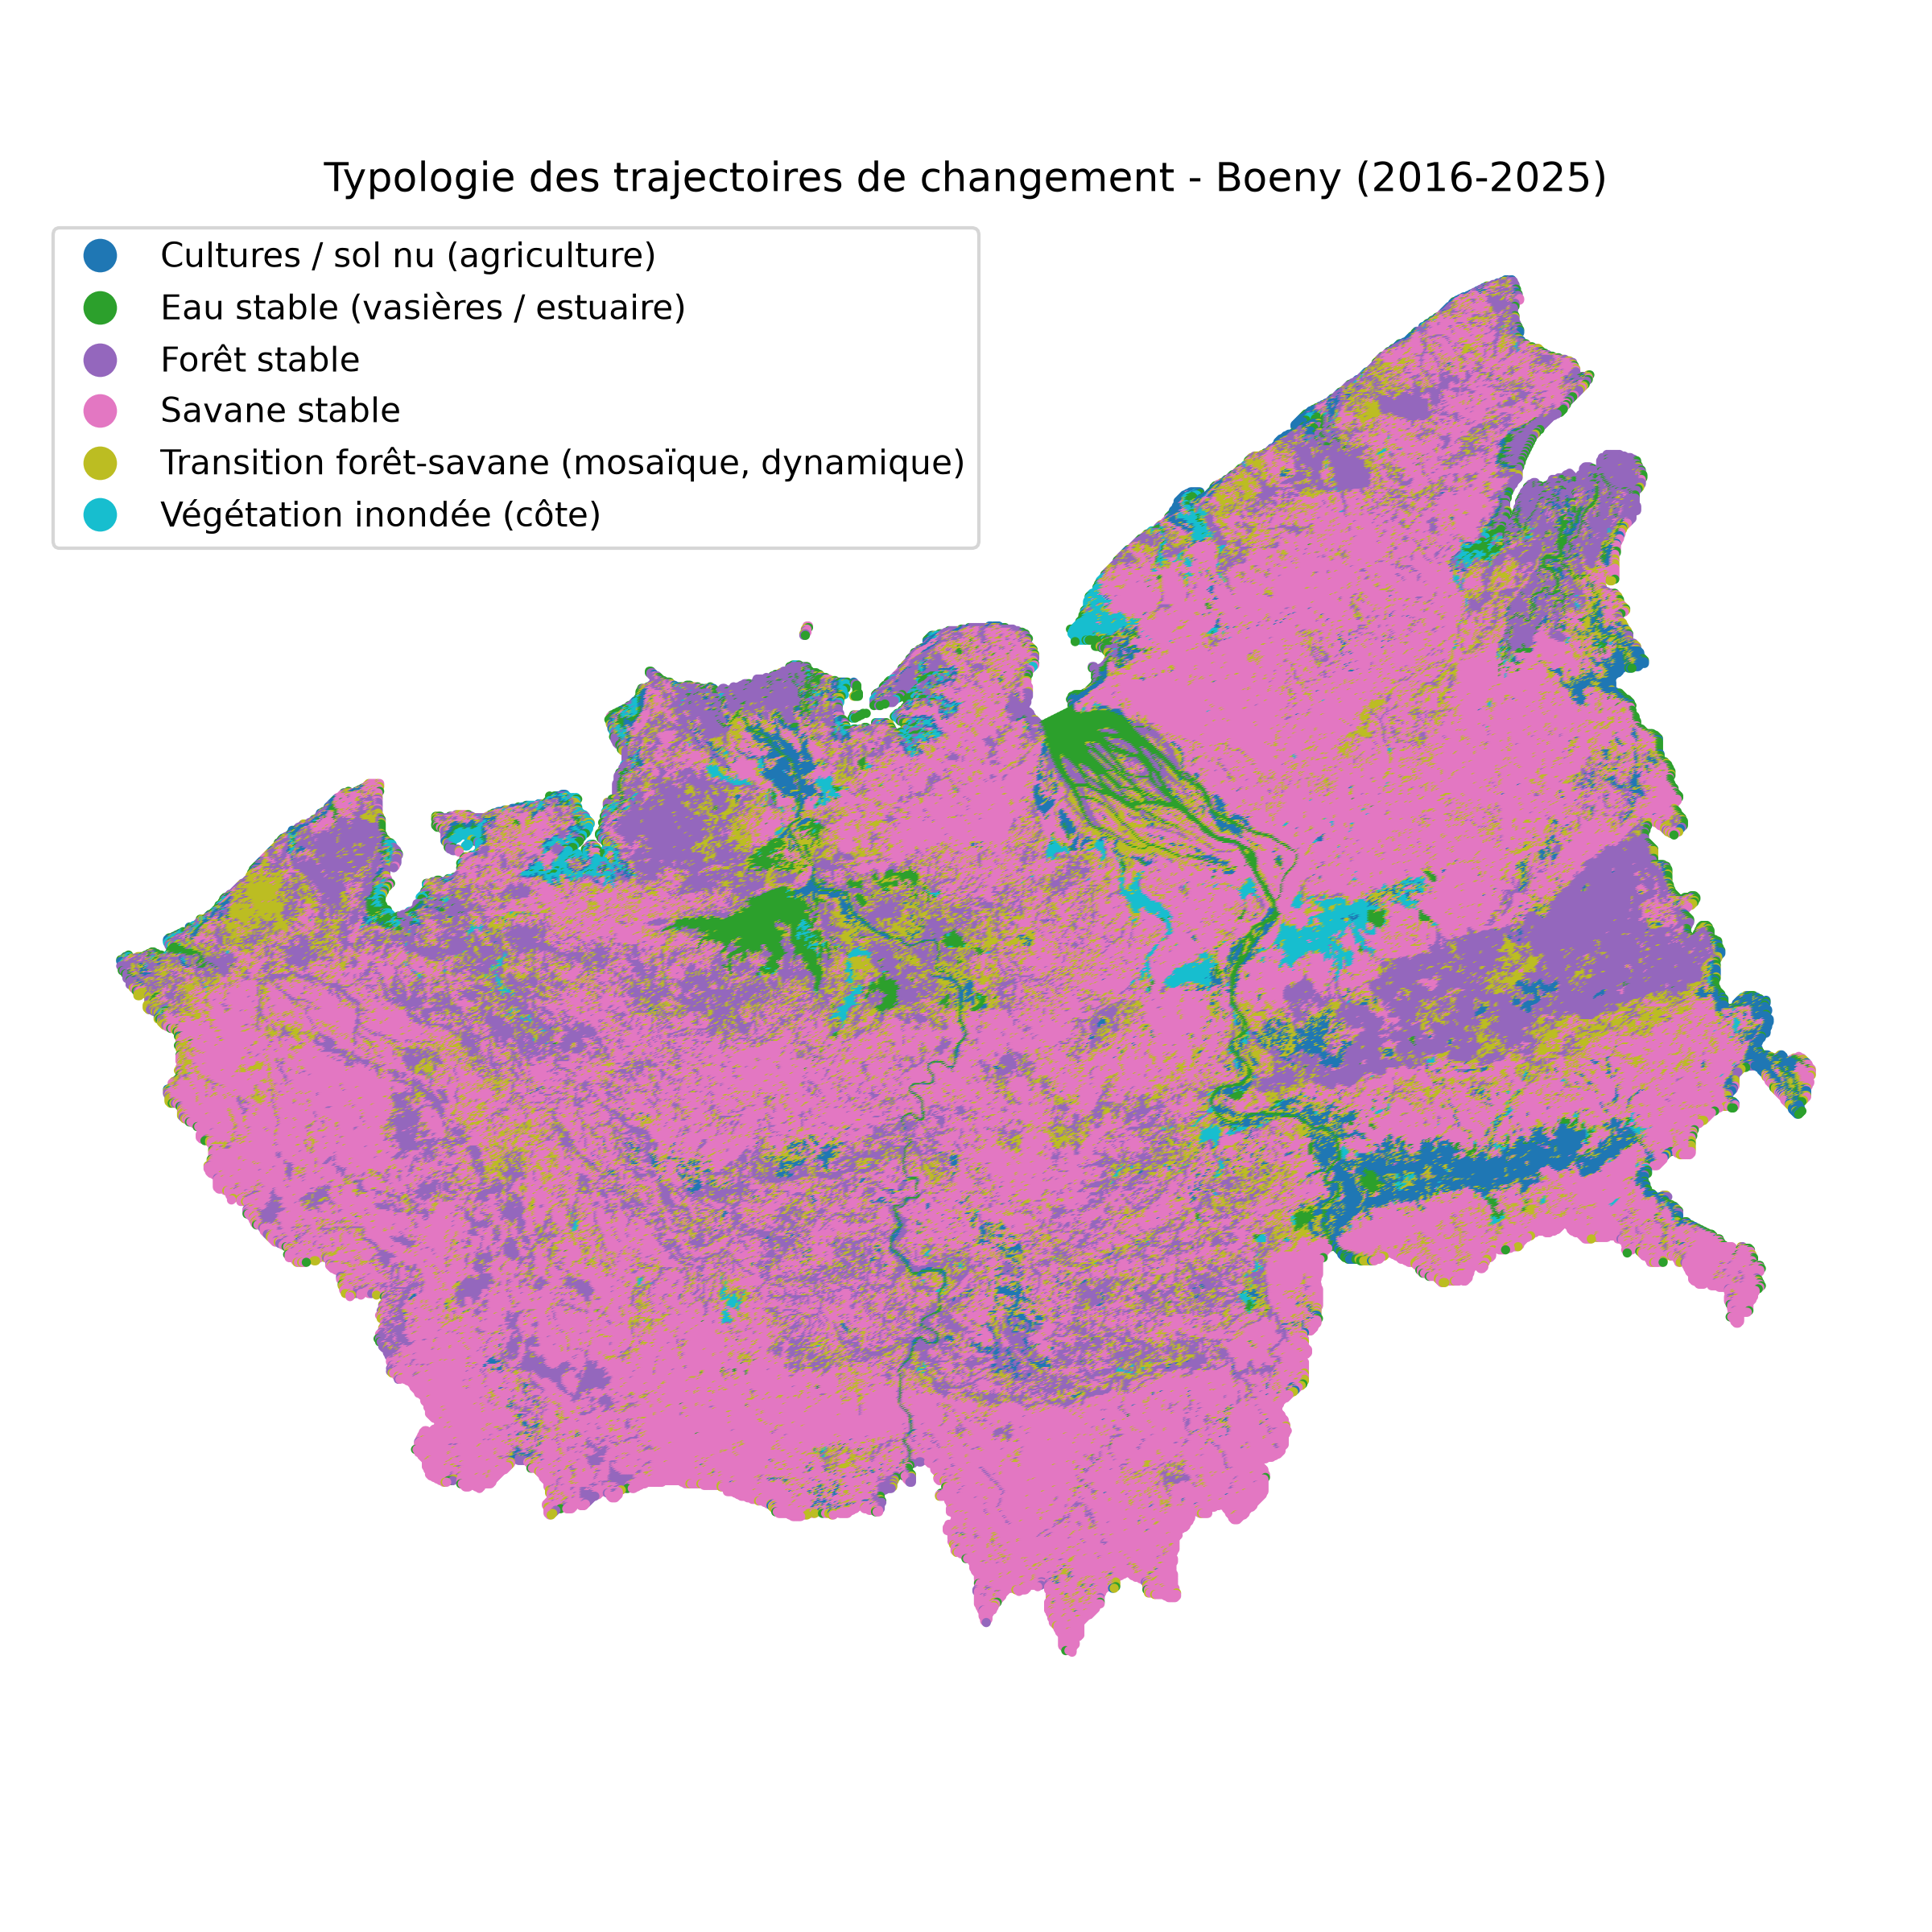
\includegraphics[width=0.85\textwidth]{carte_clusters_trajectoires.png}
\caption{Carte des trajectoires de changement (Boeny, 2016--2025), 6 clusters.}
\label{fig:carte_clusters}
\end{figure}

\section{Règles d'association sur les transitions}

L'extraction Apriori (support $\geq 0{,}01$, confiance $\geq 0{,}5$, tri par
lift) a produit 10 règles sur les \numprint{86988} cellules présentant au
moins une transition. Les plus informatives traduisent des dynamiques
spatialement localisées :

\begin{table}[H]
\centering
\caption{Principales règles d'association (extrait, tri par lift).}
\label{tab:regles_association}
\begin{tabular}{lrrrll}
\toprule
Règle (lhs $\Rightarrow$ rhs) & Support & Confiance & Lift & Effectif & Lecture \\
\midrule
eau $\Leftrightarrow$ sol nu & 0{,}010 & 0{,}56--0{,}65 & \numprint{34,9} & 899 & Vasières / estuaire (alternance annuelle) \\
vég. inondée $\Leftrightarrow$ vég. non for. & 0{,}011 & 0{,}53 & \numprint{26,7} & 914 & Frange littorale humide \\
vég. inondée $\Leftrightarrow$ forêt & 0{,}012 & 0{,}53 & \numprint{22,3} & 1007 & Bordure forêt / zone inondée \\
cultures $\Leftrightarrow$ vég. non for. & 0{,}062 & 0{,}54--0{,}62 & \numprint{5,4} & 5380 & \textbf{Front agricole} \\
forêt $\Leftrightarrow$ vég. non for. & 0{,}268 & 0{,}54--0{,}60 & \numprint{1,2} & 23307 & Co-occurrence (lift $\approx 1$, peu informative) \\
\bottomrule
\end{tabular}
\end{table}

% --- Resultat clé à mettre en avant --------------------------------
\subsection{À retenir pour le mémoire}

Deux résultats structurent le chapitre~3 : (i) l'association
\textbf{eau $\Leftrightarrow$ sol nu} (lift \numprint{34,9}) caractérise les
vasières de l'estuaire de la Betsiboka, où le marnage fait osciller la classe
d'occupation d'une année à l'autre — une dynamique côtière \emph{localisée et
intense} ; (ii) l'association \textbf{cultures $\Leftrightarrow$ vég. non
forestière} (lift \numprint{5,4}, support \SI{6,2}{\percent}) matérialise le
front agricole en bordure des espaces naturels. La règle
\textbf{forêt $\Leftrightarrow$ vég. non forestière}, bien que la plus
volumineuse (support \SI{26,8}{\percent}), est la moins informative
(lift $\approx 1{,}2$ $\approx$ indépendance) : son interprétation en terme de
dynamique doit être évitée — c'est une \emph{co-occurrence spatiale} de la
mosaïque forêt--savane à l'échelle 250 m.

% --- Section méthodologique (reproductibilité) ----------------------
\section{Reproductibilité}

L'ensemble du pipeline est reproducible avec une graine fixe
($\texttt{SEED}=1$, $\texttt{random\_state}=1$, $\texttt{nstart}=25$) et les
commandes documentées dans \texttt{GUIDE\_EXECUTION.md}. La silhouette est
calculée sur un échantillon de \numprint{5000} cellules (pratique standard en
raison du coût $O(n^2)$ du calcul complet). Le choix de $K=6$ maximise
simultanément la silhouette (\numprint{0,765}) et se situe au dernier coude
d'inertie stabilisé — deux critères indépendants convergent.

.
% Donnees : trajectoires_avec_clusters.csv (482 359 cellules), K=6, silhouette 0,765.
% Compilation : pdflatex (ou lualatex) + biblatex. Figures fournies par
% visualisation_spatiale_boeny.py / clustering_regles_association_boeny.py.
% -----------------------------------------------------------------------

\chapter{Résultats : dynamique spatio-temporelle du Boeny (2016--2025)}
\label{ch:resultats}

\section{Partition en six trajectoires types}

L'agrégation des rasters Dynamics World à 10 m vers une résolution de 250 m a
produit \numprint{482359} cellules valides sur la période 2016--2025 (masque
polygone appliqué, EPSG:32738). Après lissage (fenêtre $3\times3$ + médian
temporel, bruit ramené de \SI{16,4}{\percent} à \SI{2,0}{\percent}), un
k-means à $K=6$ — justifié par la convergence du coude d'inertie
($-20{,}7\,\%$ de 5 à 6) et de la silhouette de Rousseeuw maximale
($s=\numprint{0,765}$) — a été appliqué. La répartition est la suivante :

\begin{table}[H]
\centering
\caption{Répartition des cellules par cluster (k-means, $K=6$, 
$n_{\text{start}}=25$, silhouette $0{,}765$).}
\label{tab:repartition_clusters}
\begin{tabular}{lrrrl}
\toprule
Cluster & Cellules & \multicolumn{1}{c}{\%} & Silhouette & Lecture \\
\midrule
1 & \numprint{12909} & 2{,}7 & 0{,}166 & Eau stable (vasières / estuaire) \\
2 & \numprint{17996} & 3{,}7 & 0{,}418 & Cultures / sol nu (agriculture) \\
3 & \numprint{73390} & 15{,}2 & 0{,}796 & Transition forêt--savane (dynamique) \\
4 & \numprint{8228} & 1{,}7 & 0{,}258 & Végétation inondée (côte) \\
5 & \numprint{269063} & 55{,}8 & 0{,}000 & Savane stable \\
6 & \numprint{100773} & 20{,}9 & 0{,}000 & Forêt stable \\
\midrule
Total & \numprint{482359} & 100 & --- & --- \\
\bottomrule
\end{tabular}
\end{table}

\begin{figure}[H]
\centering
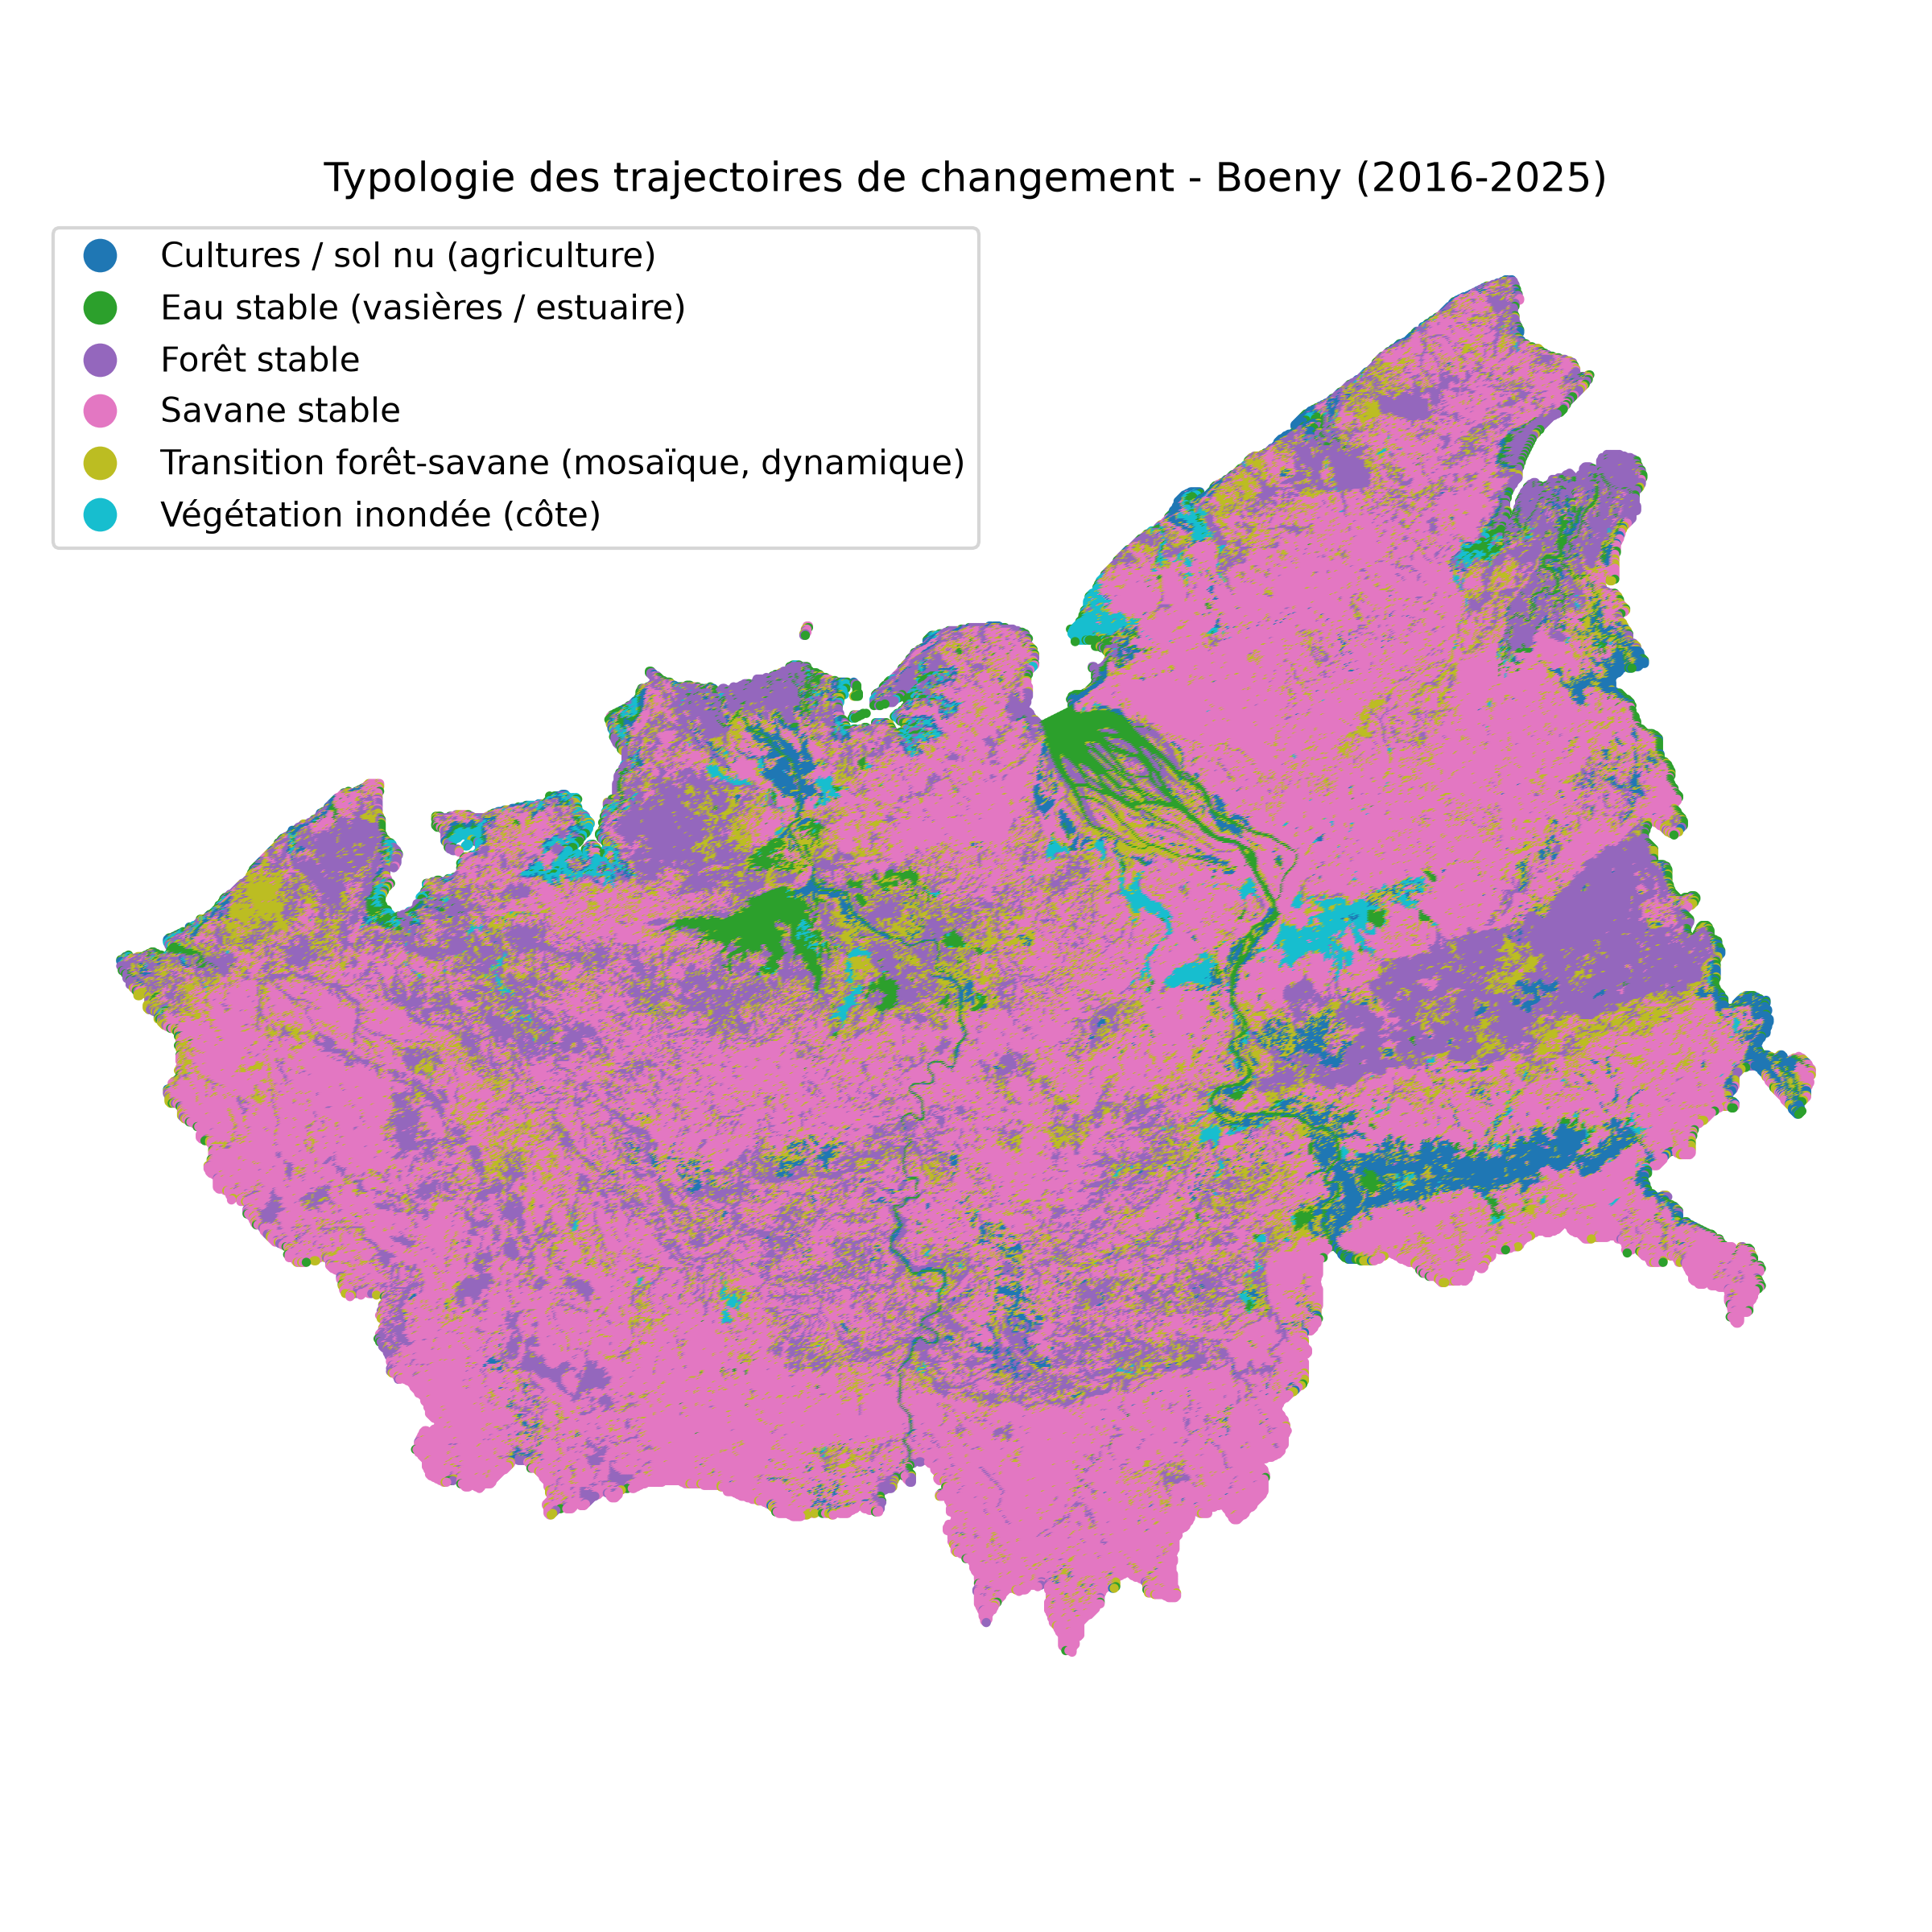
\includegraphics[width=0.85\textwidth]{carte_clusters_trajectoires.png}
\caption{Carte des trajectoires de changement (Boeny, 2016--2025), 6 clusters.}
\label{fig:carte_clusters}
\end{figure}

\section{Règles d'association sur les transitions}

L'extraction Apriori (support $\geq 0{,}01$, confiance $\geq 0{,}5$, tri par
lift) a produit 10 règles sur les \numprint{86988} cellules présentant au
moins une transition. Les plus informatives traduisent des dynamiques
spatialement localisées :

\begin{table}[H]
\centering
\caption{Principales règles d'association (extrait, tri par lift).}
\label{tab:regles_association}
\begin{tabular}{lrrrll}
\toprule
Règle (lhs $\Rightarrow$ rhs) & Support & Confiance & Lift & Effectif & Lecture \\
\midrule
eau $\Leftrightarrow$ sol nu & 0{,}010 & 0{,}56--0{,}65 & \numprint{34,9} & 899 & Vasières / estuaire (alternance annuelle) \\
vég. inondée $\Leftrightarrow$ vég. non for. & 0{,}011 & 0{,}53 & \numprint{26,7} & 914 & Frange littorale humide \\
vég. inondée $\Leftrightarrow$ forêt & 0{,}012 & 0{,}53 & \numprint{22,3} & 1007 & Bordure forêt / zone inondée \\
cultures $\Leftrightarrow$ vég. non for. & 0{,}062 & 0{,}54--0{,}62 & \numprint{5,4} & 5380 & \textbf{Front agricole} \\
forêt $\Leftrightarrow$ vég. non for. & 0{,}268 & 0{,}54--0{,}60 & \numprint{1,2} & 23307 & Co-occurrence (lift $\approx 1$, peu informative) \\
\bottomrule
\end{tabular}
\end{table}

% --- Resultat clé à mettre en avant --------------------------------
\subsection{À retenir pour le mémoire}

Deux résultats structurent le chapitre~3 : (i) l'association
\textbf{eau $\Leftrightarrow$ sol nu} (lift \numprint{34,9}) caractérise les
vasières de l'estuaire de la Betsiboka, où le marnage fait osciller la classe
d'occupation d'une année à l'autre — une dynamique côtière \emph{localisée et
intense} ; (ii) l'association \textbf{cultures $\Leftrightarrow$ vég. non
forestière} (lift \numprint{5,4}, support \SI{6,2}{\percent}) matérialise le
front agricole en bordure des espaces naturels. La règle
\textbf{forêt $\Leftrightarrow$ vég. non forestière}, bien que la plus
volumineuse (support \SI{26,8}{\percent}), est la moins informative
(lift $\approx 1{,}2$ $\approx$ indépendance) : son interprétation en terme de
dynamique doit être évitée — c'est une \emph{co-occurrence spatiale} de la
mosaïque forêt--savane à l'échelle 250 m.

% --- Section méthodologique (reproductibilité) ----------------------
\section{Reproductibilité}

L'ensemble du pipeline est reproducible avec une graine fixe
($\texttt{SEED}=1$, $\texttt{random\_state}=1$, $\texttt{nstart}=25$) et les
commandes documentées dans \texttt{GUIDE\_EXECUTION.md}. La silhouette est
calculée sur un échantillon de \numprint{5000} cellules (pratique standard en
raison du coût $O(n^2)$ du calcul complet). Le choix de $K=6$ maximise
simultanément la silhouette (\numprint{0,765}) et se situe au dernier coude
d'inertie stabilisé — deux critères indépendants convergent.

.
% Donnees : trajectoires_avec_clusters.csv (482 359 cellules), K=6, silhouette 0,765.
% Compilation : pdflatex (ou lualatex) + biblatex. Figures fournies par
% visualisation_spatiale_boeny.py / clustering_regles_association_boeny.py.
% -----------------------------------------------------------------------

\chapter{Résultats : dynamique spatio-temporelle du Boeny (2016--2025)}
\label{ch:resultats}

\section{Partition en six trajectoires types}

L'agrégation des rasters Dynamics World à 10 m vers une résolution de 250 m a
produit \numprint{482359} cellules valides sur la période 2016--2025 (masque
polygone appliqué, EPSG:32738). Après lissage (fenêtre $3\times3$ + médian
temporel, bruit ramené de \SI{16,4}{\percent} à \SI{2,0}{\percent}), un
k-means à $K=6$ — justifié par la convergence du coude d'inertie
($-20{,}7\,\%$ de 5 à 6) et de la silhouette de Rousseeuw maximale
($s=\numprint{0,765}$) — a été appliqué. La répartition est la suivante :

\begin{table}[H]
\centering
\caption{Répartition des cellules par cluster (k-means, $K=6$, 
$n_{\text{start}}=25$, silhouette $0{,}765$).}
\label{tab:repartition_clusters}
\begin{tabular}{lrrrl}
\toprule
Cluster & Cellules & \multicolumn{1}{c}{\%} & Silhouette & Lecture \\
\midrule
1 & \numprint{12909} & 2{,}7 & 0{,}166 & Eau stable (vasières / estuaire) \\
2 & \numprint{17996} & 3{,}7 & 0{,}418 & Cultures / sol nu (agriculture) \\
3 & \numprint{73390} & 15{,}2 & 0{,}796 & Transition forêt--savane (dynamique) \\
4 & \numprint{8228} & 1{,}7 & 0{,}258 & Végétation inondée (côte) \\
5 & \numprint{269063} & 55{,}8 & 0{,}000 & Savane stable \\
6 & \numprint{100773} & 20{,}9 & 0{,}000 & Forêt stable \\
\midrule
Total & \numprint{482359} & 100 & --- & --- \\
\bottomrule
\end{tabular}
\end{table}

\begin{figure}[H]
\centering
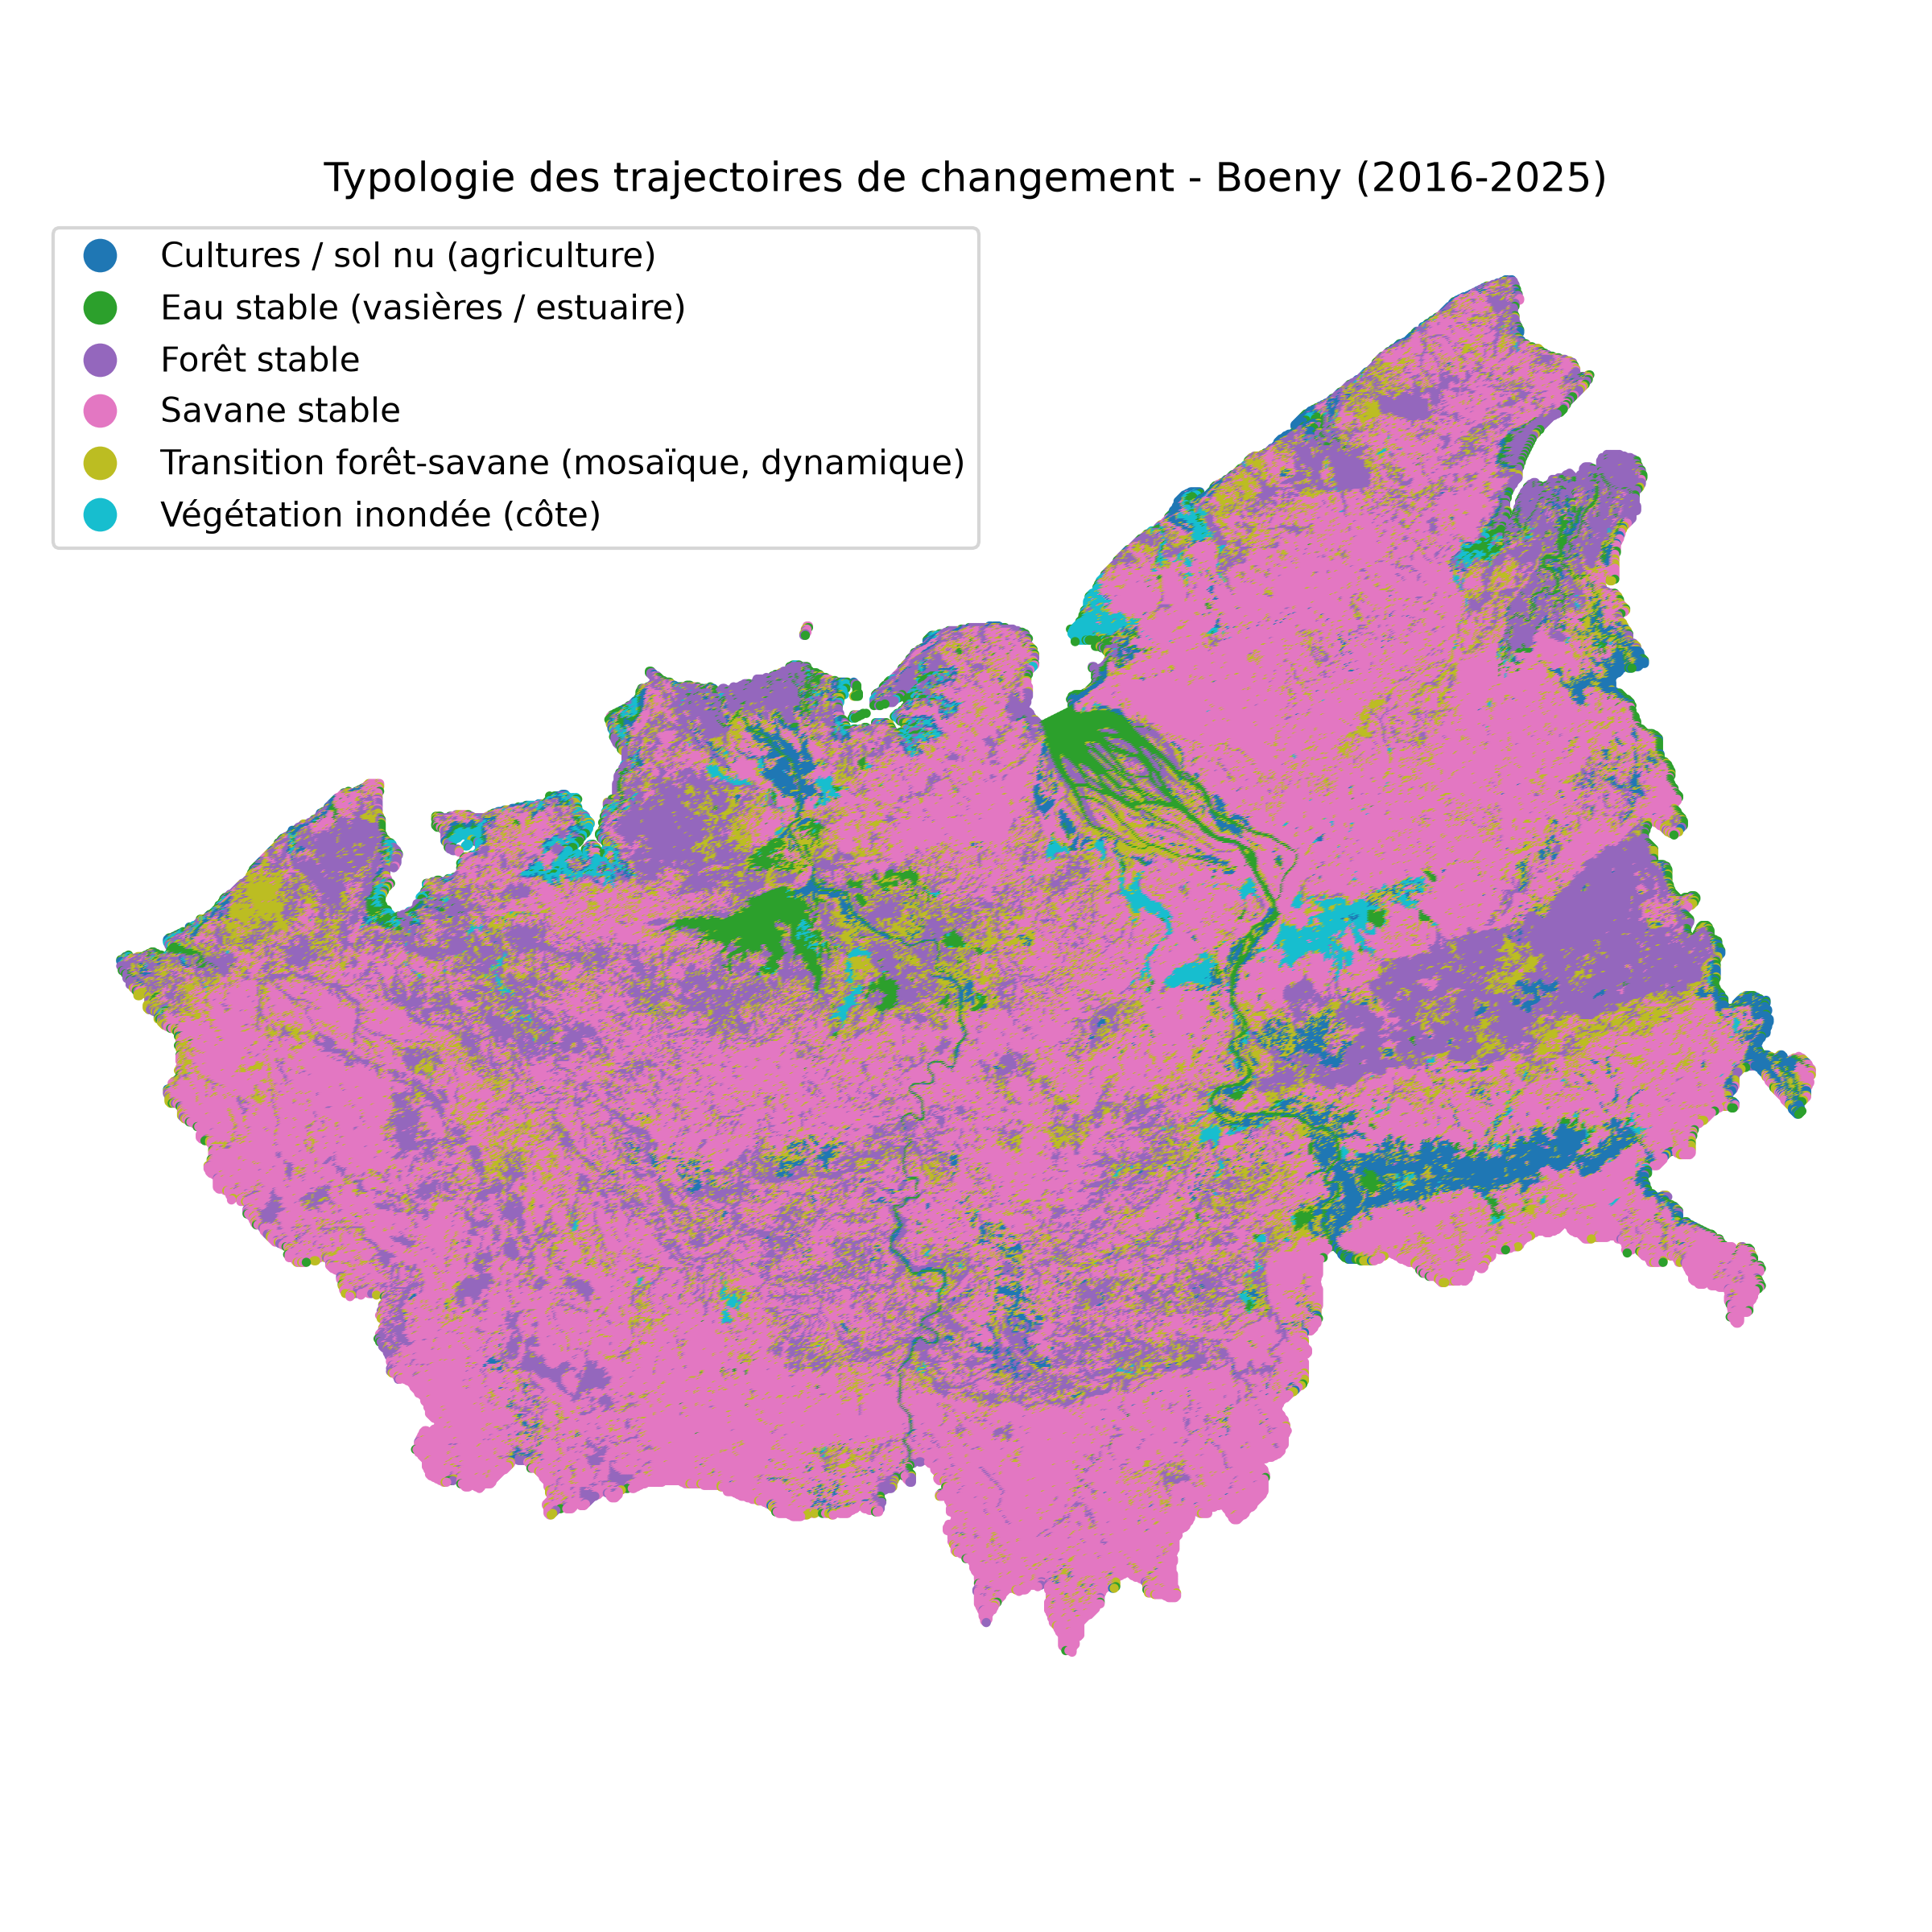
\includegraphics[width=0.85\textwidth]{carte_clusters_trajectoires.png}
\caption{Carte des trajectoires de changement (Boeny, 2016--2025), 6 clusters.}
\label{fig:carte_clusters}
\end{figure}

\section{Règles d'association sur les transitions}

L'extraction Apriori (support $\geq 0{,}01$, confiance $\geq 0{,}5$, tri par
lift) a produit 10 règles sur les \numprint{86988} cellules présentant au
moins une transition. Les plus informatives traduisent des dynamiques
spatialement localisées :

\begin{table}[H]
\centering
\caption{Principales règles d'association (extrait, tri par lift).}
\label{tab:regles_association}
\begin{tabular}{lrrrll}
\toprule
Règle (lhs $\Rightarrow$ rhs) & Support & Confiance & Lift & Effectif & Lecture \\
\midrule
eau $\Leftrightarrow$ sol nu & 0{,}010 & 0{,}56--0{,}65 & \numprint{34,9} & 899 & Vasières / estuaire (alternance annuelle) \\
vég. inondée $\Leftrightarrow$ vég. non for. & 0{,}011 & 0{,}53 & \numprint{26,7} & 914 & Frange littorale humide \\
vég. inondée $\Leftrightarrow$ forêt & 0{,}012 & 0{,}53 & \numprint{22,3} & 1007 & Bordure forêt / zone inondée \\
cultures $\Leftrightarrow$ vég. non for. & 0{,}062 & 0{,}54--0{,}62 & \numprint{5,4} & 5380 & \textbf{Front agricole} \\
forêt $\Leftrightarrow$ vég. non for. & 0{,}268 & 0{,}54--0{,}60 & \numprint{1,2} & 23307 & Co-occurrence (lift $\approx 1$, peu informative) \\
\bottomrule
\end{tabular}
\end{table}

% --- Resultat clé à mettre en avant --------------------------------
\subsection{À retenir pour le mémoire}

Deux résultats structurent le chapitre~3 : (i) l'association
\textbf{eau $\Leftrightarrow$ sol nu} (lift \numprint{34,9}) caractérise les
vasières de l'estuaire de la Betsiboka, où le marnage fait osciller la classe
d'occupation d'une année à l'autre — une dynamique côtière \emph{localisée et
intense} ; (ii) l'association \textbf{cultures $\Leftrightarrow$ vég. non
forestière} (lift \numprint{5,4}, support \SI{6,2}{\percent}) matérialise le
front agricole en bordure des espaces naturels. La règle
\textbf{forêt $\Leftrightarrow$ vég. non forestière}, bien que la plus
volumineuse (support \SI{26,8}{\percent}), est la moins informative
(lift $\approx 1{,}2$ $\approx$ indépendance) : son interprétation en terme de
dynamique doit être évitée — c'est une \emph{co-occurrence spatiale} de la
mosaïque forêt--savane à l'échelle 250 m.

% --- Section méthodologique (reproductibilité) ----------------------
\section{Reproductibilité}

L'ensemble du pipeline est reproducible avec une graine fixe
($\texttt{SEED}=1$, $\texttt{random\_state}=1$, $\texttt{nstart}=25$) et les
commandes documentées dans \texttt{GUIDE\_EXECUTION.md}. La silhouette est
calculée sur un échantillon de \numprint{5000} cellules (pratique standard en
raison du coût $O(n^2)$ du calcul complet). Le choix de $K=6$ maximise
simultanément la silhouette (\numprint{0,765}) et se situe au dernier coude
d'inertie stabilisé — deux critères indépendants convergent.

